\section{Signatures}
\begin{lstlisting}
abstract sig Bool{}
one sig True, False extends Bool {}

abstract sig Category {}
one sig A_CATEGORY, B_CATEGORY extends Category {}

abstract sig State {}
one sig FREE, RESERVED, IN_USE, OUT_OF_SERVICE extends State {}

sig Position {}
one sig SafeArea {
	coverage: set Position
}{#coverage>0}

sig ChargingStation {
	position: Position
}{position in SafeArea.coverage}

abstract sig BatteryLevel {}
one sig LOW, MEDIUM, HIGH extends BatteryLevel {}

abstract sig Vehicle {
	category: one Category,
	state: one State,
	position: one Position,
	batteryLevel: one BatteryLevel,
	plugged: one Bool
}{
	batteryLevel = LOW implies state = OUT_OF_SERVICE 
	not (position in SafeArea.coverage) implies state=OUT_OF_SERVICE
	plugged=True implies ( position in SafeArea.coverage)
}
sig Car extends Vehicle{}{category=B_CATEGORY}

sig License{
	categories: set Category
}{#categories>0}

sig User {
	license: one License,
	isLocked: one Bool
}

abstract sig BillType {}
one sig EXPIRATION_BILL, STD_BILL, DISCOUNT_BILL, FEE_BILL extends BillType {}  
sig Bill {
	type: one BillType,
	payed: one Bool   
}

abstract sig Event {
	user: one User,
	vehicle: one Vehicle,
	startTime: one Int,
	endTime: lone Int
}{
	startTime>0
	#endTime=1 implies endTime>startTime
}

sig Reservation extends Event{
	isExpired: one Bool,
	bill: lone Bill
}{
	isActive[this] implies isExpired=False
	isExpired=True implies not isActive[this]
	#bill=1 <=> isExpired=True 
	#bill=1 implies bill.type=EXPIRATION_BILL
}

sig Ride extends Event{
	reservation: one Reservation,
	startPosition: one Position,
	endPosition: lone Position,
	hasAdditionalPassengers: one Bool,
	hasLeftLowBattery: one Bool,
	hasLeftHighBattery: one Bool,
	hasLeftPlugged: one Bool,
	bill: lone Bill
}{
	startPosition in SafeArea.coverage
	startPosition!=endPosition
	hasLeftHighBattery=True <=> not hasLeftLowBattery=True
	#bill=1 <=> #endPosition=1
	#endPosition=1 <=> not isActive[this]
	bill.type!=EXPIRATION_BILL
 	bill.type=DISCOUNT_BILL <=> not isActive[this] and (endPosition in SafeArea.coverage) and (hasAdditionalPassengers=True or hasLeftHighBattery=True or hasLeftPlugged=True)
 	bill.type=FEE_BILL <=> not isActive[this] and not bill.type=DISCOUNT_BILL and (not(endPosition in SafeArea.coverage) or hasLeftLowBattery=True)
	bill.type=STD_BILL <=> not isActive[this] and not bill.type=DISCOUNT_BILL and not bill.type=FEE_BILL
}
\end{lstlisting}
\section{Facts}
\begin{lstlisting}
// all reservations are assigned to at most one ride and have coherent user/vehicle
fact ReservationMatchRide {
	all res:Reservation | lone ride:Ride | ride.reservation=res
    all ride:Ride | ride.user=ride.reservation.user
	all ride:Ride | ride.vehicle=ride.reservation.vehicle
}

// no more active events from the same user
fact NoEventOverlap {
	no disj e1, e2:Event | overlap[e1, e2] and e1.user=e2.user 
	no disj e1, e2:Event | overlap[e1, e2] and e1.vehicle=e2.vehicle 
}

// all licenses belong to one user
fact LicenseMatchUser {
	all l:License | one u:User | u.license=l
}

// users cannot reserve/drive vehicles without the correct license 
fact LicenseMatchVehicle {
	all e:Event | e.vehicle.category in e.user.license.categories
}

// all rides must have a valid reservation associated
fact NoRandomRide {
	no r:Ride | isActive[r.reservation]
	no r:Ride | r.reservation.isExpired=True
	all ride:Ride | ride.startTime>=ride.reservation.endTime
}

// banned users cannot reserve/drive cars
fact NoLockedUserAction {
	no r:Reservation | isActive[r] and r.user.isLocked=True
}

// vehicle state should be consistent
fact VehicleStateConsistency {
	all v:Vehicle | v.state=FREE or v.state=OUT_OF_SERVICE implies (no e:Event | e.vehicle=v and isActive[e])
	all v:Vehicle | v.state=RESERVED implies (one r:Reservation | r.vehicle=v and isActive[r])
	all v:Vehicle | v.state=IN_USE implies (one r:Ride | r.vehicle=v and isActive[r])
}

// all bills are assigned to a ride or a reservation
fact NoRandomBill {
	all b:Bill | one r1:Reservation, r2:Ride | r1.bill=b or r2.bill=b
}

//if vehicle was used its position should match with last ride endPosition
fact ConsistentVehiclePosition {
	all v:Vehicle | (some r:Ride | r.vehicle=v) implies (some r1:Ride | (r1.endPosition=v.position) and (all r2:Ride | r2!=r1 and r2.vehicle=r1.vehicle implies r2.endTime<r1.endTime))  
}

//if vehicle was used its plugging state should match with last ride plugging state
fact ConsistentVehiclePlugging {
	all r:Ride | some c:ChargingStation | r.hasLeftPlugged=True implies r.endPosition=c.position
	all v:Vehicle | (some r:Ride | r.vehicle=v) implies (some r1:Ride | (r1.hasLeftPlugged=True <=> v.plugged=True) and (all r2:Ride | r2!=r1 and r2.vehicle=r1.vehicle implies r2.endTime<r1.endTime))
}

//if vehicle was used its batteryLevel should match with last ride batteryLevel
fact ConsistentVehicleBattery {
	all v:Vehicle | (some r:Ride | r.vehicle=v) implies (some r1:Ride | (r1.hasLeftHighBattery=True <=> v.batteryLevel=HIGH) and (all r2:Ride | r2!=r1 and r2.vehicle=r1.vehicle implies r2.endTime<r1.endTime))  
	all v:Vehicle | (some r:Ride | r.vehicle=v) implies (some r1:Ride | (r1.hasLeftLowBattery=True <=> v.batteryLevel=LOW) and (all r2:Ride | r2!=r1 and r2.vehicle=r1.vehicle implies r2.endTime<r1.endTime))  
	all v:Vehicle | (some r:Ride | r.vehicle=v) implies (some r1:Ride | (r1.hasLeftHighBattery=False and r1.hasLeftLowBattery=False <=> v.batteryLevel=MEDIUM) and (all r2:Ride | r2!=r1 and r2.vehicle=r1.vehicle implies r2.endTime<r1.endTime))
}

// no two distinct objects with the same position
fact ConsistentPosition {
	no disj v1,v2:Vehicle | v1.position = v2.position
	no disj c1,c2:ChargingStation | c1.position = c2.position
}
\end{lstlisting}
\section{Predicates}
\begin{lstlisting}
pred isActive [e: Event]{
	#e.endTime=0
}

pred overlap [e1,e2: Event]{
	e1.startTime<e2.startTime and e2.startTime<e1.endTime or 
	e2.startTime<e1.startTime and e1.startTime<e2.endTime or
	isActive[e1] and isActive[e2]
}

pred show {}
\end{lstlisting}
\section{Results}
Executing "Run show for 3"
   Solver=sat4j Bitwidth=4 MaxSeq=3 SkolemDepth=1 Symmetry=20
   5642 vars. 302 primary vars. 13223 clauses. 151ms.
   Instance found. Predicate is consistent. 49ms.
\section{Generated World}
\subsubsection{Sequence diagram}
\begin{figure}[!ht]
  \centering
  \vspace{0.2cm}
  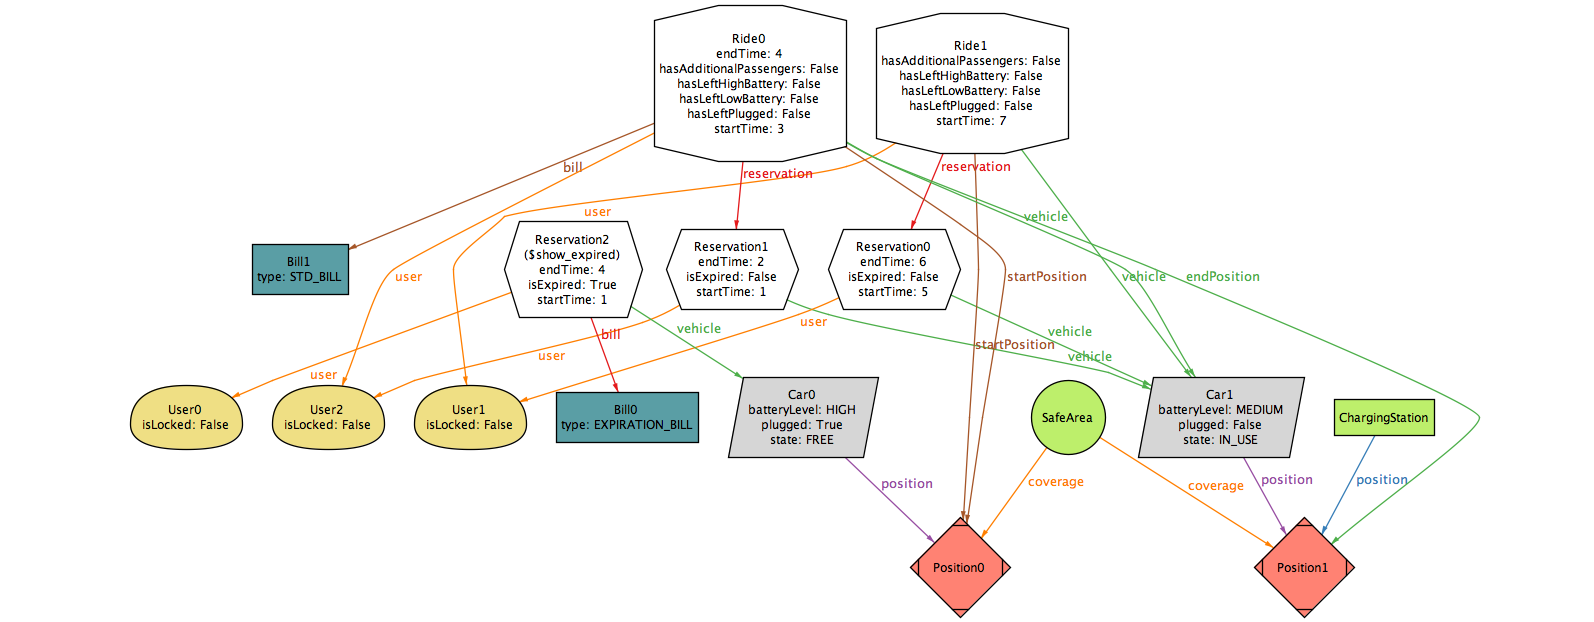
\includegraphics[width=0.6\textwidth]{/RASD/alloy_world}\\
  \vspace{0.2cm}
  %\caption{Sequence diagram for the alloy world} 
  \label{fig:alloy_world} 
\end{figure}
